\documentclass{article}
\usepackage{graphicx} % Required for inserting images

\title{Milestone One}
\author{Team 2}
\date{February 2024}

\begin{document}

\maketitle

\section{Introduction}
The purpose of this document is to express our findings and understanding of what the first milestone asks for. The milestone is split into two parts; task one instructs the team to read through a paper and summarize our findings. The second task is to perform Exploratory Data Analysis(EDA) on the data set used.
\section{Task One}
\subsection{Background}
The paper, \textit{DrugOrchestra: Jointly predicting drug response, targets, and side effects via deep multi-task learning }, was written by researchers at Stanford University and focuses on predicting drug response, targets, and side effects. The researchers created Drug Orchestra. Drug Orchestra uses a deep learning multi task learning(MTL) model to assist in pharmacogenomics. Pharmacogenomics is the study of how a person’s genes affect their response to drugs. The importance of this field stems from safety; the creation of a medical drug that is safe for all to use and has minimal side effects is the end goal. The key idea of MTL is to solve multiple prediction tasks at the same time while automatically exploiting similarities and differences across tasks. This predicts drug response, targets, and side effects. It address the predicting of drug response, drug targets, and drug side effects in pharmacogenomics. Their proposed  idea is Drug Orchestra which is a multi-task learning method that predicts drug respond, targets and side effects.
\subsection{Datasets}
The data sets used to create Drug Orchestra was sourced from many locations and serve different purposes. The datasets for the prediction of drug responses include target DTI’s (drug-response interactions) from Repurposing Hub, Drugbank, and STITCH, drug response data from a Patient-Derived Xenograft dataset (PDX), the Genomics of Drug Sensitivity in Cancer database (GDSC), and the Cancer Therapeutics Response Portal database (CCLE), and finally the drug side effects were pulled from the SIDER and OFFSIDES databases, with a relation between the being drawn utilizing DisGeNET, which contains associations between genome data and diseases.
\subsection{Model}
The DrugOrchestra is an MTL. An MTL works by doing multiple tasks at once as opposed to one at a time. This can be seen in figure 2 where each task specific layer occurs at the same time in unison. Neural networks are used as the basis for prediction and control the shared layers. The model provides further classification using the sigmoid function in a Rectified Linear Unit function. The Rectified Linear Unit function is an activation function that will occur once a certain threshold has crossed. In DrugOrchestra's case, the two input features for each task will be evaluated and then if the sigmoid reaches a certain threshold, the activation will occur taking in the sigmoid's data.
\subsection{Results}
After the experiment was concluded the researchers found that seven out of eight datasets obtained significant improvement compared to other models. The models in comparison are Support Vector Machines (SVM), Random Network, and Single Task Learning Neural Networks (STLNN). DrugOrchestra boasted higher metric scores on all the data sets except for PDX where SVM was slightly higher. STLNN performed well as well and had close metric scores within the margin of error similar to DrugOrchestra; AUROC metrics using stitch for example. Table four shows that the researchers observed four out of six task pairs had positive performance gain by using DrugOrchestra. This works well in the model's favor because the comparison models had negative gain when focusing on the transferability between side effect and target datasets. This shows that DrugOrchestra can work well using other datasets beyond the experiment.
\section{Task Two}
The second task was to perform EDA. There were many files from each data set listed in the Standford report. The two versions of the data drive was a summarized version and a much longer raw version. The raw version contained columns of float values that led to different categories to aid in training the model. The raw versions were incredibly large files, figure 1, as well. Due to memory issues from how large the files were, EDA had to be done on the broken up pieces of the raw data and the summarized version. The number plots of the data are categorical in nature and does not have a higher or lower instance with its given numbering. The drug embedding file contains the drug SMILES. The distribution for the different response is outlined in figure one. The box plot represents the different SMILES that behavior. 
\begin{figure}
    \centering
    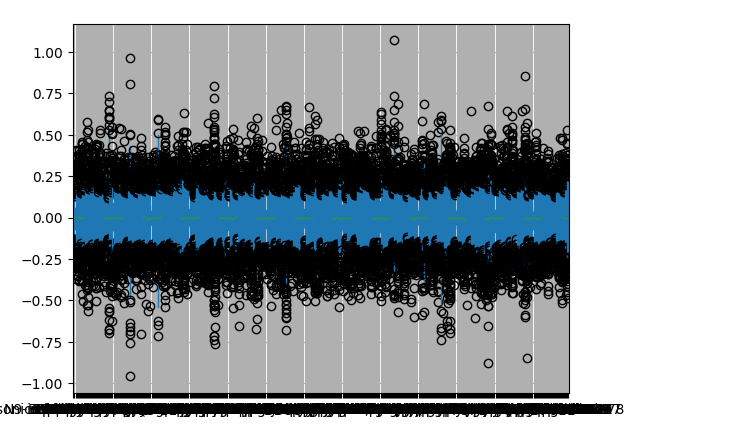
\includegraphics[width=0.5\linewidth]{a.png}
    \caption{SMILES Box Plot}
    \label{fig:enter-label}
\end{figure}
The relationship between separate drug types were also explored to determine if correlation could help train the model. However, in the example case between MST-312 and GSK4112, there is low correlation. Therefore it would be improbable to train the model using correlation in some cased for assistance as displayed in figure two.
\begin{figure}
    \centering
    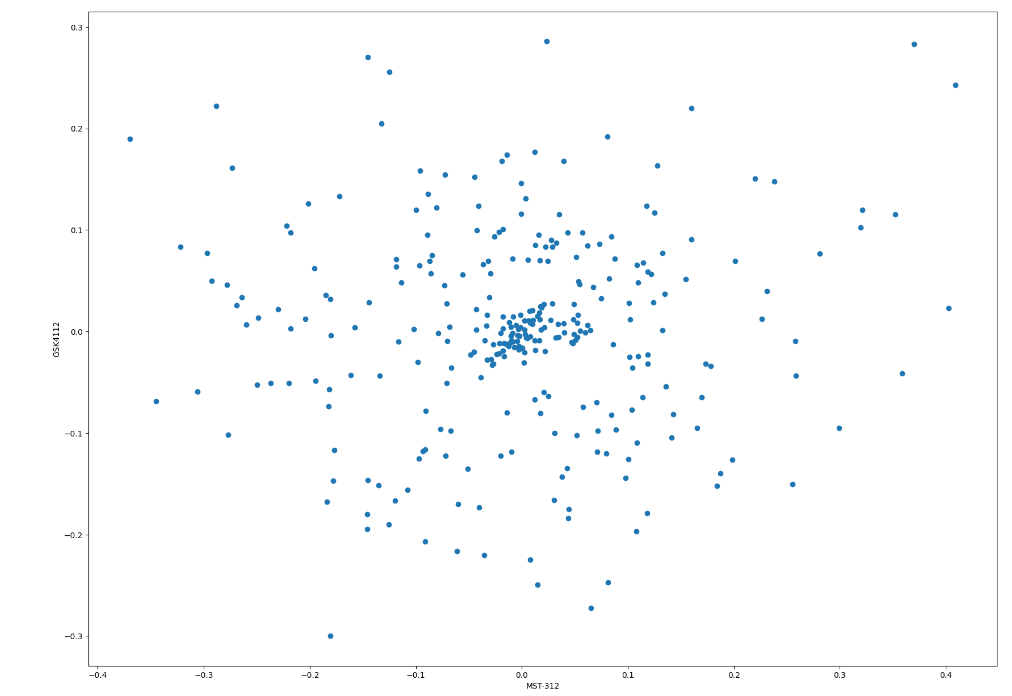
\includegraphics[width=0.5\linewidth]{b.png}
    \caption{Scatter plot a}
    \label{fig:enter-label}
\end{figure}
CCL features had EDA conducted on them as well. In the example figure three, the features are specific parts of their respective organs, and the drug that was targeted to it. Although it is not stated what each categorical number means, the correlation between the two in the example shows some correlation and can assist in training the model to make a case for both targeted outcomes. 
\begin{figure}
    \centering
    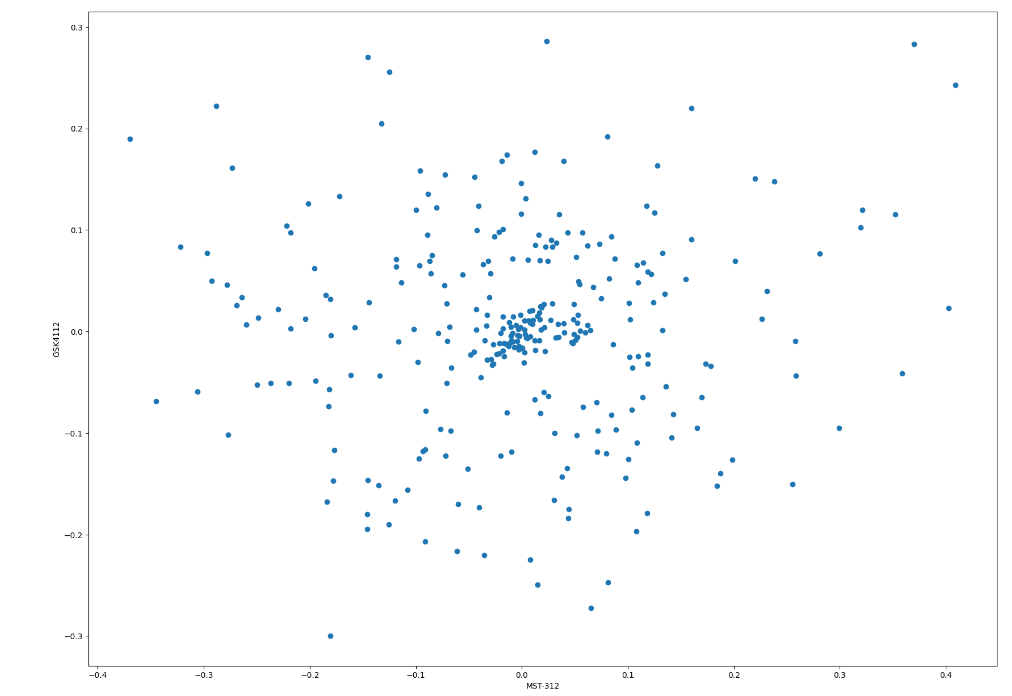
\includegraphics[width=0.5\linewidth]{c.png}
    \caption{Scatter plot b}
    \label{fig:enter-label}
\end{figure}
The side effect dataset, same as the others, contains categorical numbers. However, the values have other meaning beyond just values, it helps act as a classifier for further guessing along the span of all of the predictions. This shows true with the rest of the data sets.
\section{Conclusion}
The purpose of this milestone was to understand and summarize a research paper and conduct EDA on the data used to to create that paper. EDA showed that the distribution of data the researchers used to create Drug Orchestra would better train it using decision trees. Furthermore, it would handle and better predict response, target, and side effects of drugs given a type of gene set. The milestone proved useful in practicing EDA on larger, more complex, real world data sets.
\end{document}
